\chapter{Using the HBase Java API}
%Intro\footnotemark\\
\par HBase provides an API in Java to be able to manipulate database data. We will show here a
simple example.
\begin{spacing}{1.2}
%note en bas de page
\section{Configure the CLASSPATH in the .bashrc }
\par To compile our java code without problems, you must include the Hbase libraries in the default classpath,
thanks to the \$CLASSPATH environment variable, for this:
\\
\begin{figure}[!htb] 
\begin{center} 
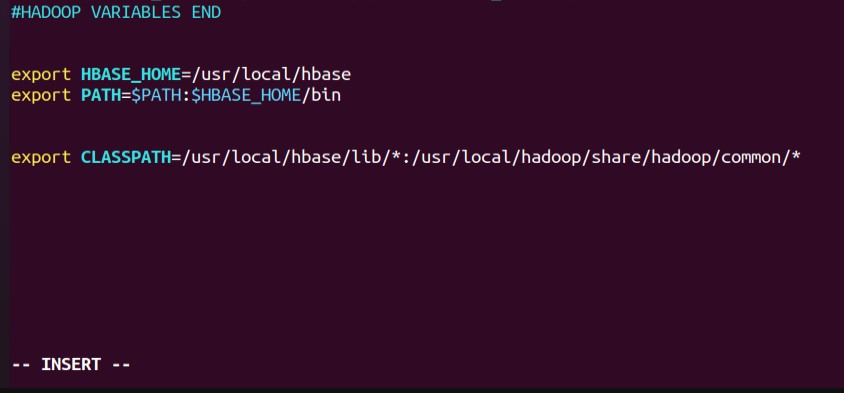
\includegraphics[width=1\linewidth]{Pictures/HBase/Using the HBase Java API/Configure the CLASSPATH in the .bashrc/Adding classpath in .bashrc} 
\end{center} 
\caption{Adding classpath in .bashrc} 
\end{figure}  \FloatBarrier
\\
\newpage

\par Creating a new hbase-code repository in the Documents folder.
\\
\begin{figure}[!htb] 
\begin{center} 
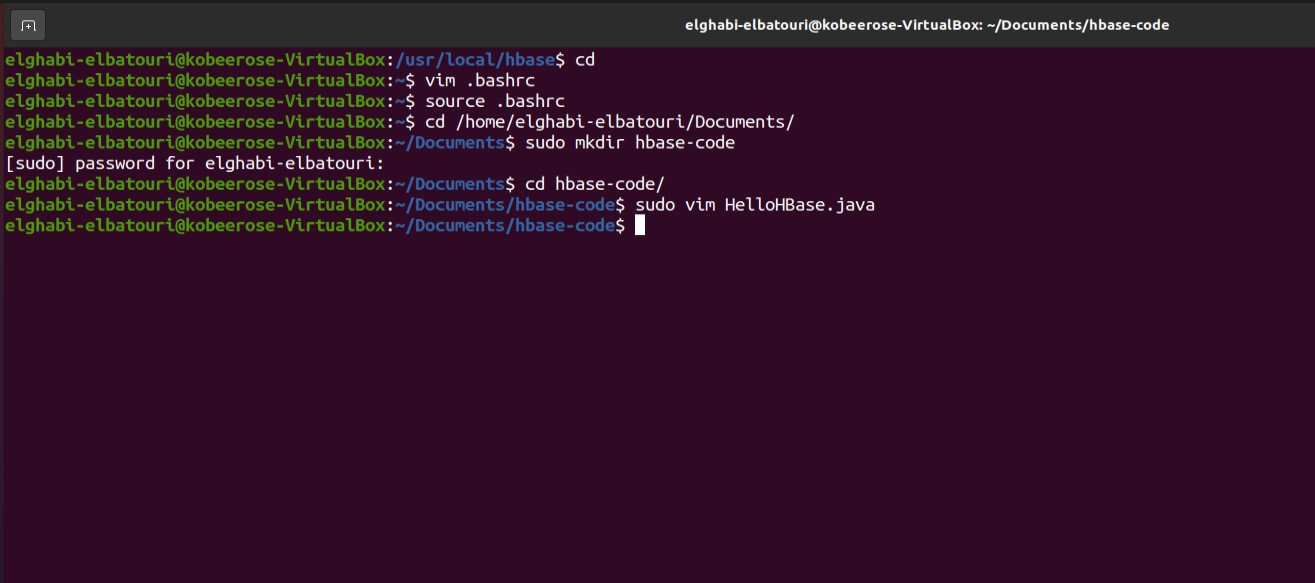
\includegraphics[width=1\linewidth]{Pictures/HBase/Using the HBase Java API/Configure the CLASSPATH in the .bashrc/Creating hbase-code repository} 
\end{center} 
\caption{Creating hbase-code repository} 
\end{figure}  \FloatBarrier
\\

\par Creating “HelloHBase.java” file which contains code that will perform the following operations:
\begin{itemize}
  \item Create a table called "user" containing two families of columns: "PersonalData" and
"ProfessionalData". If this table already exists, it will be overwritten.
  \item Insert two records in this table.
  \item Read the value of the 'PersonalData:name' column of the 'user1' row.
\end{itemize}

\\
\begin{figure}[!htb] 
\begin{center} 
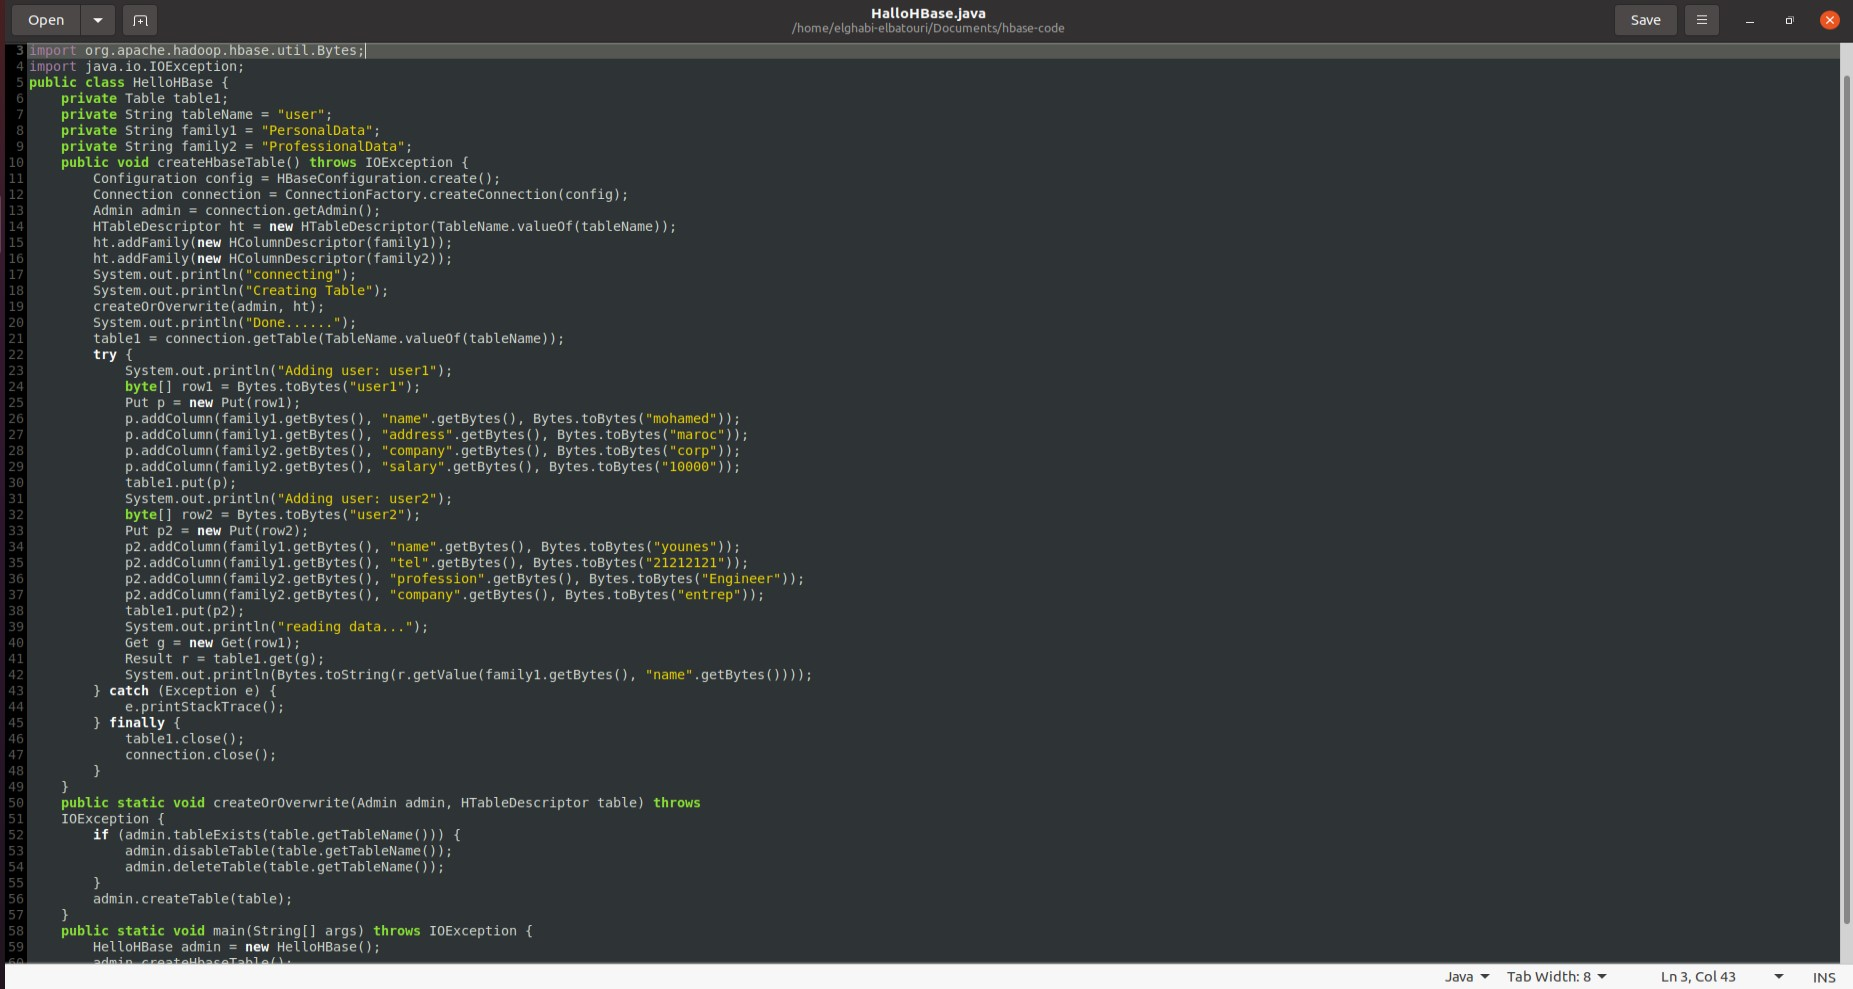
\includegraphics[width=1\linewidth]{Pictures/HBase/Using the HBase Java API/Configure the CLASSPATH in the .bashrc/HelloBase.java code} 
\end{center} 
\caption{HelloBase.java code} 
\end{figure}  \FloatBarrier
\\
\newpage
\par Compiling and running the “HelloHBase.java” class.
\\
\begin{figure}[!htb] 
\begin{center} 
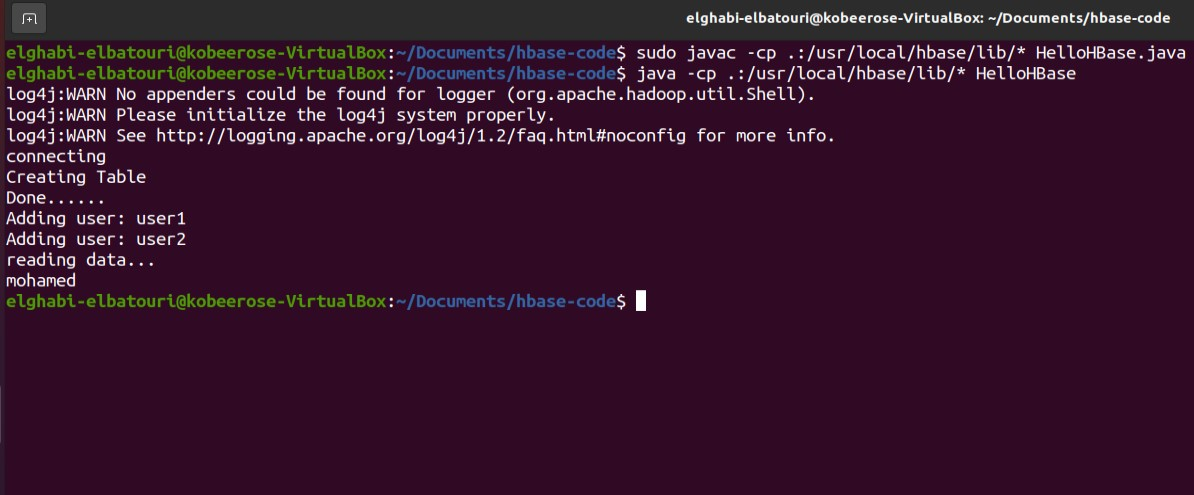
\includegraphics[width=1\linewidth]{Pictures/HBase/Using the HBase Java API/Configure the CLASSPATH in the .bashrc/Compile and run the Class} 
\end{center} 
\caption{Compile and run the Class} 
\end{figure}  \FloatBarrier
\\


\section{MapReduce on stored file }
\par We start by loading the file into the input directory of HDFS that we should first create.
\\
\begin{figure}[!htb] 
\begin{center} 
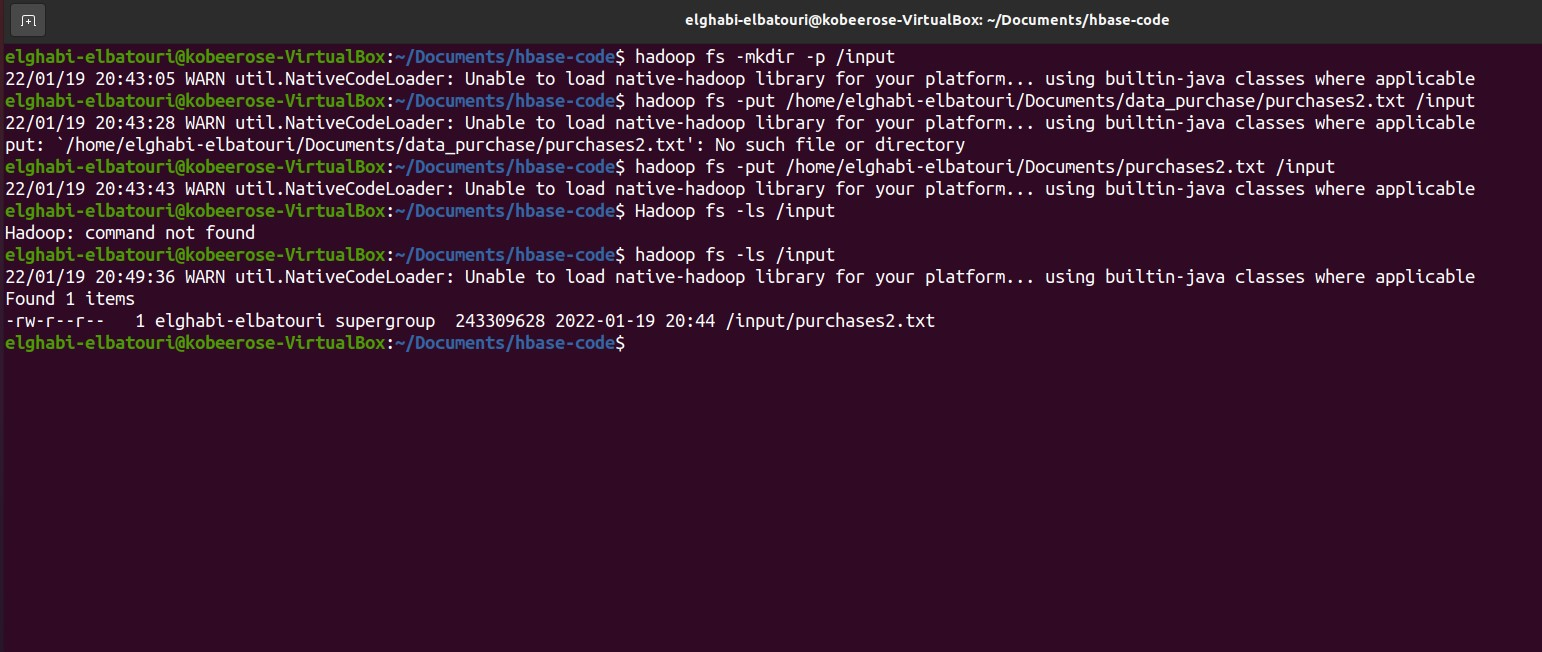
\includegraphics[width=1\linewidth]{Pictures/HBase/Using the HBase Java API/MapReduce on stored file/Putting the file into HDFS directory} 
\end{center} 
\caption{Putting the file into HDFS directory} 
\end{figure}  \FloatBarrier
\\
\newpage
\par Creating the products database with a family of 'cf' columns.
\\
\begin{figure}[!htb] 
\begin{center} 
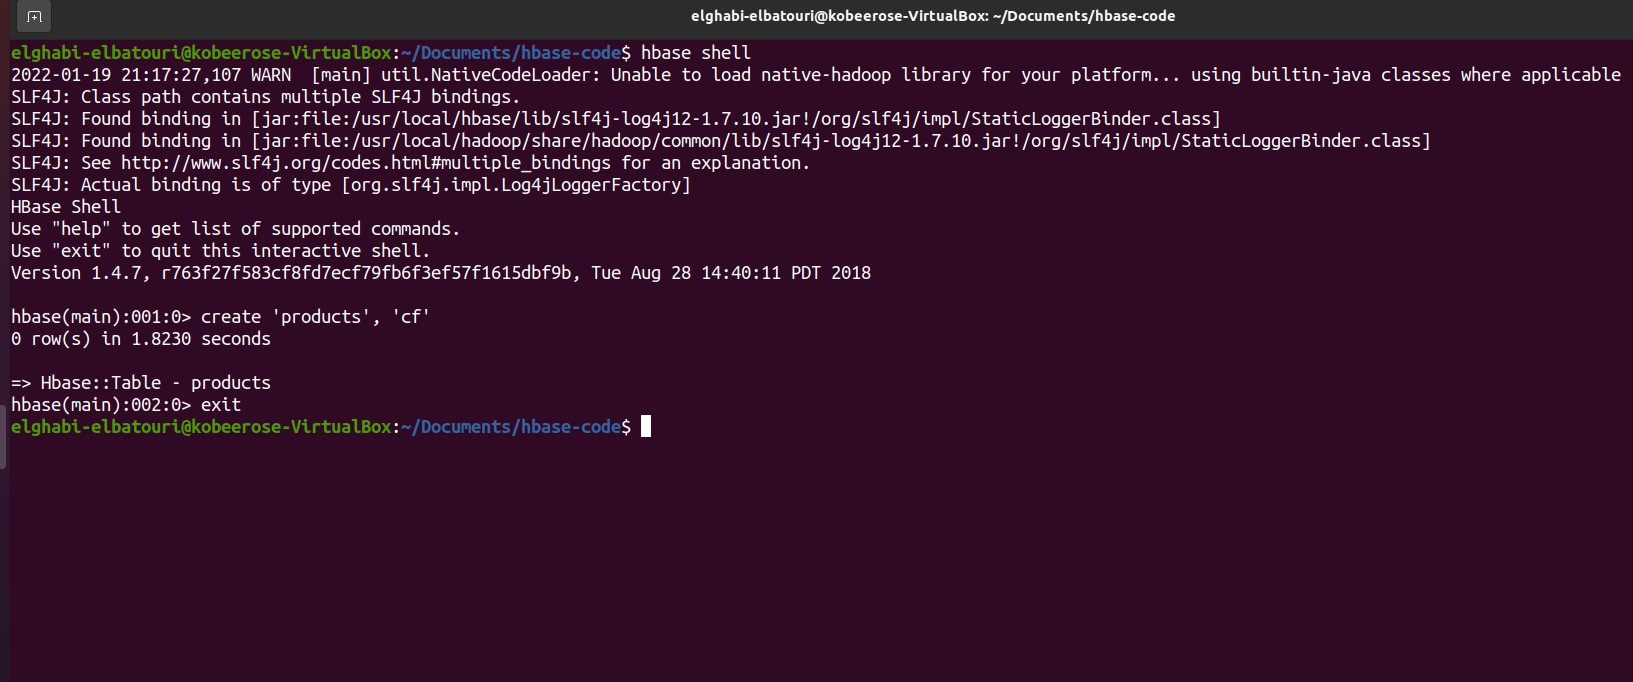
\includegraphics[width=1\linewidth]{Pictures/HBase/Using the HBase Java API/MapReduce on stored file/Create product database} 
\end{center} 
\caption{Create product database} 
\end{figure}  \FloatBarrier
\\

\par Now let's trigger a MapReduce operation on the main file stored in
HDFS, to read the data then insert them via puts into the database.
\\
\begin{figure}[!htb] 
\begin{center} 
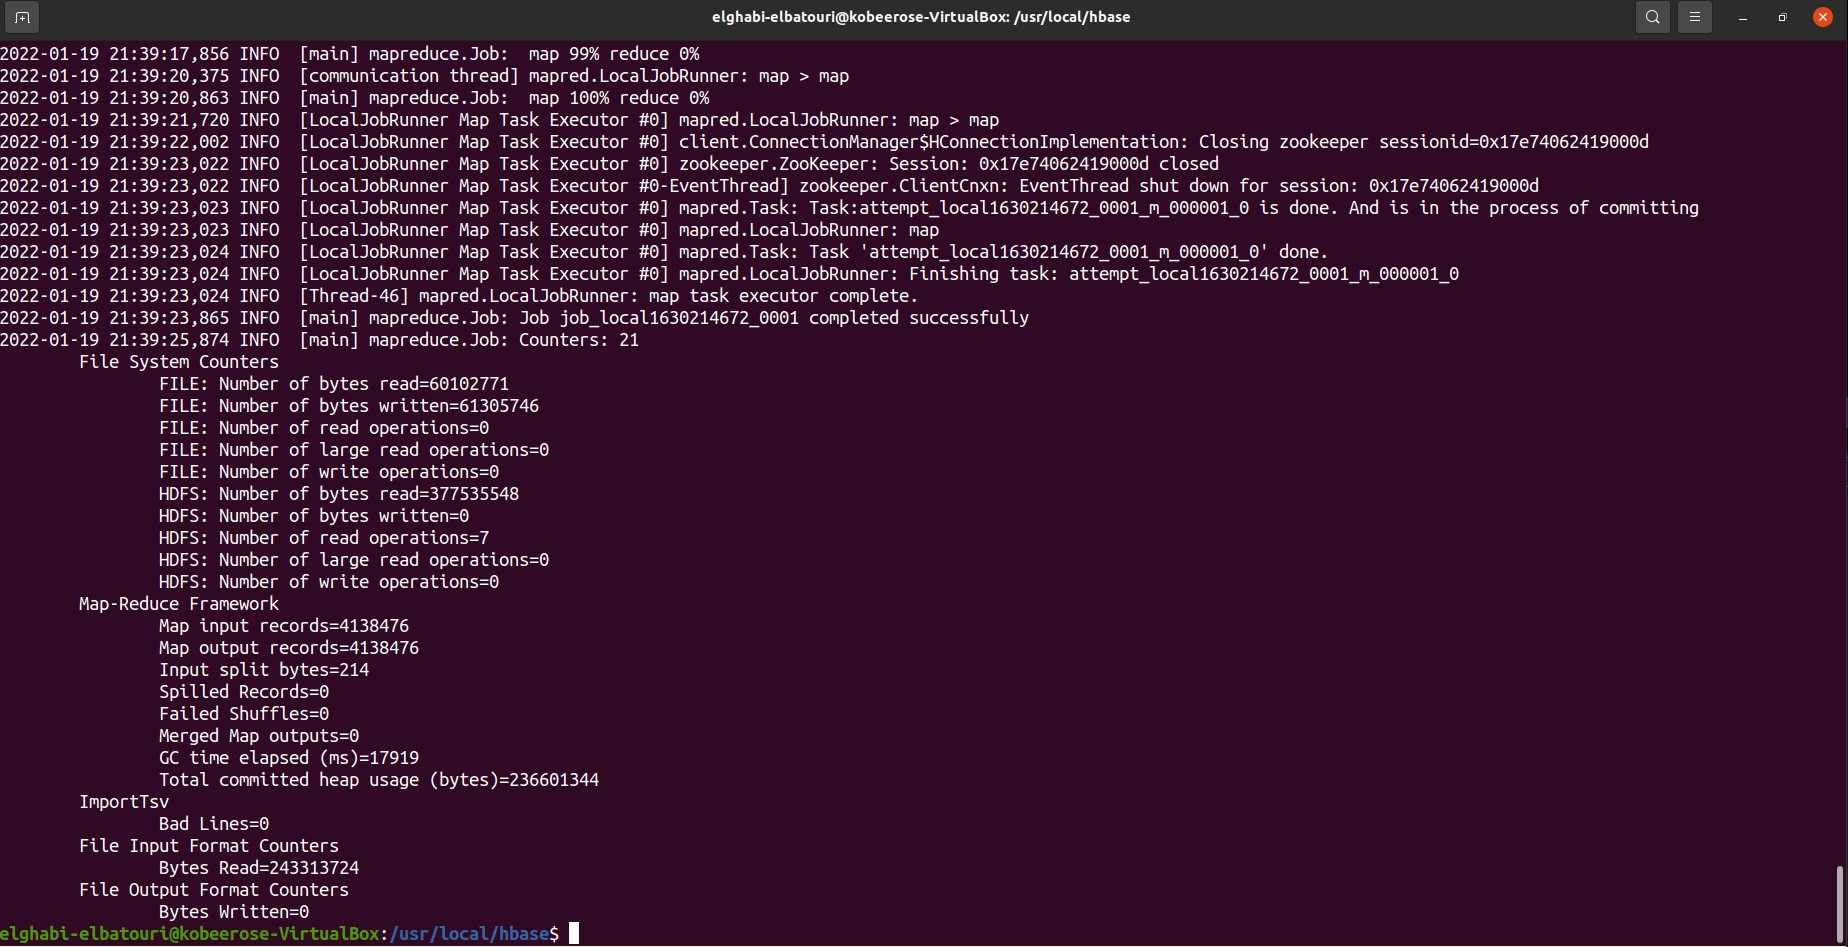
\includegraphics[width=1\linewidth]{Pictures/HBase/Using the HBase Java API/MapReduce on stored file/MapReduce on the stored file} 
\end{center} 
\caption{MapReduce on the stored file} 
\end{figure}  \FloatBarrier
\\
\newpage
\par we finally Check that the database has been created by consulting the city of record number 2000:
\\
\begin{figure}[!htb] 
\begin{center} 
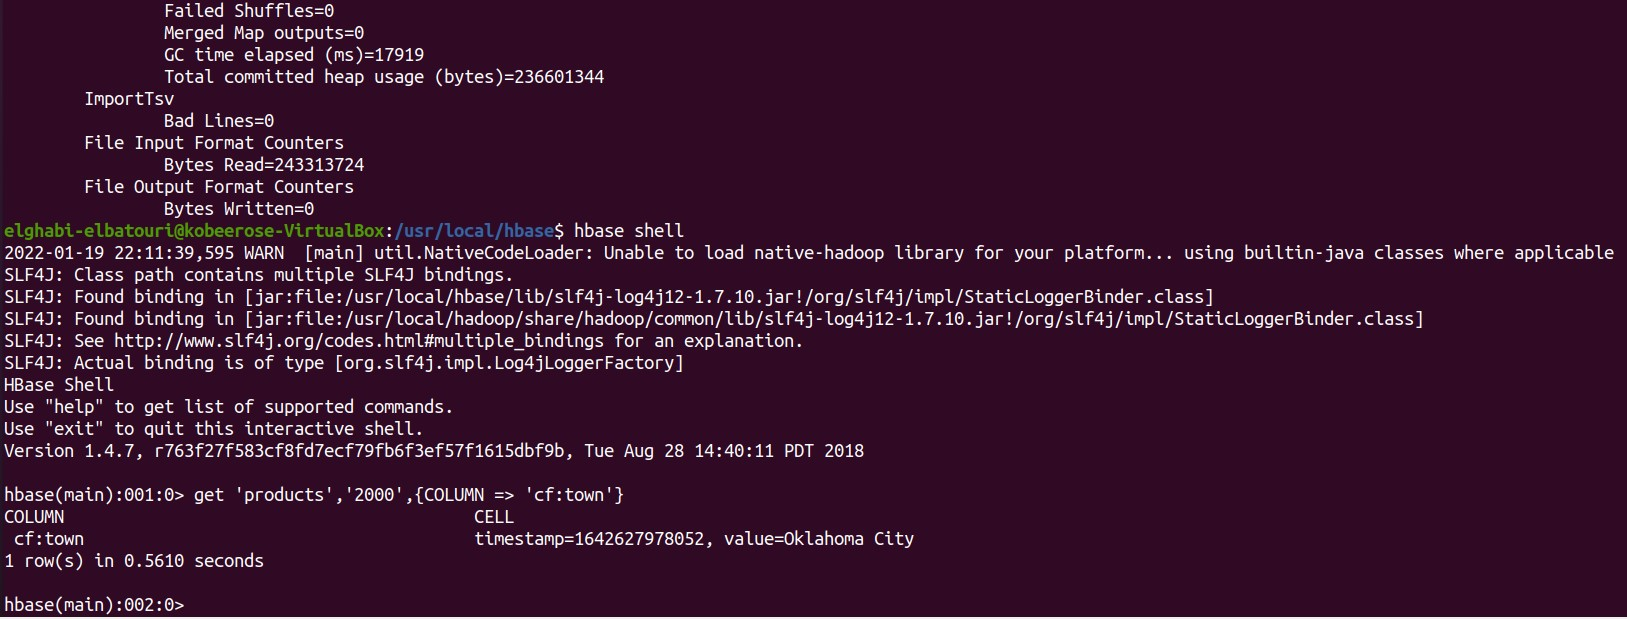
\includegraphics[width=1\linewidth]{Pictures/HBase/Using the HBase Java API/MapReduce on stored file/Verifying the Database} 
\end{center} 
\caption{Verifying the Database} 
\end{figure}  \FloatBarrier
\\

\end{spacing}